\documentclass{../notatki}

\title{Kompresja danych}

\begin{document}

\tableofcontents

\section{Wstęp}

Wyróżniamy dwa rodzaje kompresji. W kompresji stratnej dopuszczalny jest pewien
stopień straty informacji wejściowej. W kompresji bezstratnej nie jest to
dopuszczalne.

\subsection{"Prawo" Kompresji bezstratnej}

\textbf{Nie istnieje algorytm, który potrafi zmniejszyć rozmiar
dowolnych danych}

\begin{itemize}
  \item Kompresja bezstratna musi być bijekcją
  \item Dowolne dane przyjmują postać ciągu bitów długości $n$. Jest
    $2^n$ takich ciągów.
  \item Danych krótszych niż $n$, np.: o jeden jest $2^{n - 1}$
  \item Nie da się stworzyć bijekcji z zbioru o mocy $2^n$ do zbioru o
    mocy $2^{n - 1}$
\end{itemize}
Wniosek jest taki, że koniecznym jest konstruowanie kompresji bezstratnej na
podzbiorach danych, takich jak np.: obrazów, dźwięków, tekstów.

\section{Teoria informacji}

Teoria informacji to dziedzina zajmująca się przetwarzaniem informacji.
W teorii informacji mamy do czynienia z podstawowym założeniem, że zdarzenia
niosą ze sobą pewną ilość informacji. Im rzadsze zdarzenie, tym bardziej
informacyjne. Można to sobie wyobrazić jako zaskoczenie, jakie niesie ze sobą
dane zdarzenie. Zaskoczenie wynikające, z tego że wstało słońce, jest mniejsze
niż zaskoczenie wynikające z tego, że konkretny autobus się spóźnił.

\subsection{Miara informacji}

Miarą informacji, którą niesie ze sobą zdarzenie $A$ jest:
$$
I(A) = -\log_xP(A)
$$
gdzie $x$ to baza systemu liczbowego. Jeśli miarą informacji jest bit to $x=2$.
Jeśli zdarzenia $A$ i $B$ są niezależne to:
$$
I(AB) = I(A) + I(B)
$$

\subsection{Entropia}

Entropia to miara średniej informacji przekazywanej przez źródło.
Kody jednoznacznie dekodowalne w modelu z niezależnymi
wystąpieniami symboli muszą mieć średnią długość co najmniej
równą entropii.

\subsubsection{Entropia źródła}

Dla źródła danych $S$ generującego ciąg $X$ nad alfabetem
$\mathcal{A}=\{1, 2, \dots m\}$

$$
H(S) = \lim_{n \to \infty} \frac{G_n}{n}
$$
$$
G_n = - \sum_{i} \dots \sum_{j}P(X_1 = i, \dots, X_n = j) \log P(X_1
= i, \dots, X_n = j)
$$

\subsubsection{Entropia Pierwszego Rzędu}

Dla źródła informacji $X$, z zbiorem wiadomości (zdarzeń) $A_1, \dots, A_n$,
gdzie $P(A_i)$ to prawdopodobieństwo wystąpienia zdarzenia $A_i$ i
zdarzenia są niezależne to entropia źródła to:
$$
H(X) = \sum_{i=1}^{n}P(A_i)I(A_i)
$$

\section{Kodowanie}

Kodowanie to przyporządkowanie elementom jakiegoś alfabetu ciągu binarnych.
Przykładami kodowania są: ASCII, UTF-8 oraz inne. Typowym jest konstruowanie
kodowania pod konkretny zestaw danych, optymalizując je pod kątem częstości
występowania poszczególnych elementów.

\subsection{Modelowanie danych}

Rozważmy ciąg: $a_n=9,11,11,11,14,13,15,17,16,17,20,21$. $\max(a_n)=21$ stąd
koniecznym jest 5 bitów na element. Ale jeśli wykorzystamy wzór
$e_n=a_n - n + 8$ do stworzenia nowego ciągu, to ten ciąg przyjmuje postać:
$0,1,0,-1,1,-1,0,1,-1,-1,1,1$. Teraz wystarczą tylko 2 bity na zakodowanie
elementu.

\subsection{Średnia długość kodu}

$$
I = \sum_{i=1}^{n}p_i \cdot l_i
$$
gdzie $p_i$ to prawdopodobieństwo wystąpienia elementu $i$, a $l_i$ to długość
kodu dla elementu $i$.

\subsection{Jednoznaczna dekodowalność}

Jeśli dla dowolnego ciągu znaków istnieje tylko jedno jego rozkodowanie to
kod jest jednoznacznie dekodowalny. Aby sprawdzić czy kod jest jednoznacznie
dekodowalny, należy zastosować następujący algorytm.

\begin{enumerate}
  \item Stwórz pustą listę
  \item Dla każdej pary słów kodowych sprawdź czy jedno jest prefiksem
    drugiego. Jeśli tak, dodaj sufiks drugiego słowa do listy, jeśli
    już go tam nie ma.
  \item Jeśli na liście jest słowo kodowe, to kod nie jest jednoznacznie
    dekodowalny.
\end{enumerate}

\subsubsection{Nierówność Krafta}

Jeżeli $\mathcal{C}$ jest kodem jednoznacznie dekodowalnym z $n$ słowami to:
$$
K(\mathcal{C}) = \sum_{i=1}^{n}2^{-l_i} \leq 1
$$
Jest to warunek konieczny bycia kodem jednoznacznie dekodowalnym.

\subsubsection{Kod prefiksowy}

Kod w którym żadne słowo kodowe nie jest prefiksem innego słowa
kodowego. Wszystkie kody prefiksowe są jednoznacznie dekodowalne.

\subsection{Kod natychmiastowy}

Jest kodem pozwalającym stwierdzić w którym miejscu zakończone jest
słowo kodowe w momencie odczytania ostatniej litery.

\section{Kompresja bezstratna}

Z reguły kompresja bezstratna opiera się na stworzeniu kodu, który
pozwala na zakodowanie będące krótsze niż oryginalne dane. W tym celu
wykorzystuje się różne techniki kodowania.

\subsection{Statyczny Kod Huffmana}

Kod Huffmana to kod prefiksowy o minimalnej średniej długości kodu.
Są one optymalne wśród kodów prefiksowych.

Dla alfabetu $\mathcal{A}$ o długości $n$ i prawdopodobieństwach
wystąpienia $p_1, \dots, p_n$ algorytm tworzenia kodu Huffmana wygląda
następująco:
Znajdź dwa najrzadziej występujące elementy i połącz je w jeden element
o prawdopodobieństwie $p_1 + p_2$. Rozróżnij je $0$ lub $1$. Powtórz
ten krok na liście $n-1$ długiej aż zostanie jeden element.

\begin{figure*}[h]
  \centering
  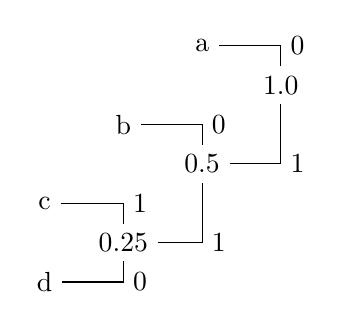
\begin{tikzpicture}
    \node (d) at (0, 0) {d};
    \node (c) at (0, 1) {c};
    \node (c_d) at (1, 0.5) {$0.25$};
    \node (b) at (1, 2) {b};
    \node (b_c_d) at (2, 1.5) {$0.5$};
    \node (a) at (2, 3) {a};
    \node (a_b_c_d) at (3, 2.5) {$1.0$};

    \draw[-] (d) -| (c_d) node[midway, right] {0};
    \draw[-] (c) -| (c_d) node[midway, right] {1};

    \draw[-] (b) -| (b_c_d) node[midway, right] {0};
    \draw[-] (c_d) -| (b_c_d) node[midway, right] {1};

    \draw[-] (a) -| (a_b_c_d) node[midway, right] {0};
    \draw[-] (b_c_d) -| (a_b_c_d) node[midway, right] {1};
  \end{tikzpicture}
  \caption{Przykład kodu Huffmana dla $P(a) = 0.5, P(b) = 0.25, P(c)
  = 0.15, P(d) = 0.1$}
\end{figure*}

\subsection{Kodowanie Shannon-Fano}

Dla symboli $a_1, \dots, a_n$ o prawdopodobieństwach $p_1, \dots, p_n$,
ustalmy kody długości $l_n = \lceil - \log p_i \rceil$. Następnie
zdefiniujmy zmienne pomocnicze $w_1, \dots w_n$ jako:
$$
w_1 = 0, w_j = \sum_{i=1}^{j-1}2^{l_j - l_i}
$$
Jeżeli $\lceil \log w_j \rceil = l_j$ to j-te słowo kodowe jest binarną
reprezentacją $w_j$. Jeżeli $\lceil \log w_j \rceil < l_j$ to reprezentację
uzupełniamy zerami z lewej strony.

Dla $P(a) = \frac{1}{3}, P(b) = \frac{1}{4}, P(c) = \frac{1}{4}, P(d)
= \frac{1}{6}$ mamy:
$$
l_a = 2, l_b = 2, l_c = 2, l_d = 3
$$
$$
w_1 = 0, w_2 = 2, w_3 = 2, w_4 = 6
$$
$$
kod(a) = 00, kod(b) = 01, kod(c) = 10, kod(d) = 110
$$

\subsection{Kodowanie Tunstalla}

Chcemy stworzyć kod na $n$ bitach dla $a_1, \dots, a_m$ symboli o
prawdopodobieństwach $p_1, \dots, p_m$. Tworzenie kodu Tunstalla polega na
iteracyjnym wyborze ze zbioru symbolu o największym prawdopodobieństwie $S$
i łączenie go z wszystkimi innymi symbolami tworząc symbole $Sa_m$, nadając im
prawdopodobieństwa $P \cdot p_m$. Proces ten powtarzamy aż do uzyskania
kodu o długości $n$.

\subsection{Kodowanie Golomba}

Kody Golomba są parametryzowane liczbą $m > 0$. Każda liczba $n$ jest zapisywana
za pomocą $q = \lfloor \frac{n}{m} \rfloor$ oraz $r = n - q \cdot m$ w postaci
$$
(q)_1(r)_2
$$

\subsection{Dynamiczne kodowanie Huffmana}

Głównym problemem kodowania Huffmana jest konieczność znania całego ciągu
danych przed rozpoczęciem kodowania. Rozwiązaniem tego problemu jest
dynamiczne kodowanie, gdzie stosujemy kodowanie Huffmana dla $k + 1$ symbolu
na podstawie kodowania dla $k$ symboli. W tym celu tworzymy dynamicznie drzewo,
gdzie każdy liść ma wagę równą ilości wystąpień danego symbolu. Drzewo zaczyna
się od liścia z symbolem \texttt{EOF} o wadze $0$.

\newcommand{\drawNode}[3]{
  \node[draw] (#1) at (#3) {#2};
  \node[below] at (#1.south) {\texttt{#1}};
}

\begin{figure}[H]
  \centering
  \resizebox{0.8\textwidth}{!}{
    \begin{minipage}{0.25\textwidth}
      \begin{tikzpicture}
        \drawNode{EOF}{0}{0,0}
      \end{tikzpicture}
    \end{minipage}
    \begin{minipage}{0.25\textwidth}
      \begin{tikzpicture}
        \drawNode{EOF}{0}{0,0}
        \drawNode{a}{1}{1,0}
        \node[circle, draw] (root) at (0.5, 1) {1};
        \draw[-] (root) -- (a);
        \draw[-] (root) -- (EOF);
      \end{tikzpicture}
    \end{minipage}
    \begin{minipage}{0.25\textwidth}
      \begin{tikzpicture}
        \drawNode{EOF}{0}{0,0}
        \drawNode{r}{1}{1,0}
        \node[circle, draw] (root2) at (0.5, 1) {1};
        \draw[-] (root2) -- (r);
        \draw[-] (root2) -- (EOF);
        \drawNode{a}{1}{2,1}
        \node[circle, draw] (root) at (1.25, 2) {2};
        \draw[-] (root) -- (root2);
        \draw[-] (root) -- (a);
      \end{tikzpicture}
    \end{minipage}
  }
  \caption{Przykład kodowania dynamicznego}
\end{figure}

\subsection{Problem kodowania uniwersalnego}

Szukamy sposobu na kodowanie dowolnej liczby $n \in \mathbb{N}$. Problem polega
na skonstruowaniu kodu, który będzie jednoznacznie dekodowalny i uniwersalny.
To oznacza, że ma się skalować w nieskończoność.

\subsubsection{Kodowanie Eliasa}

Kodowanie Eliasa to kodowanie uniwersalne, które wykorzystuje kodowanie unarne
do zapisania długości kodu binarnego liczby $n$.

$$
n = \lfloor \log_2(x) \rfloor + 1
$$

\paragraph{$\gamma$}

Jest to najprostsze z kodowań Eliasa. Polega na zakodowaniu liczby $x$ w
postaci binarnej, a następnie dodaniu przed nią liczby $n-1$ zer.

$$
\gamma(x) = 0^{n-1}(x)_2
$$
$$
(13)_{10} = 1101_2 \Rightarrow \gamma(13) = 0001101
$$

\paragraph{$\delta$}

Cały trik kodu $\delta$ polega na zakodowaniu długości kodu binarnego liczby
$x$ przy pomocy kodu $\gamma$.
Istotnym trikiem jest usunięcie najstarszego bitu z zakodowanej liczby $x$.

$$
\delta(x) = \gamma(n) + (x)_2
$$
$$
(13)_{10} = 1101_2 \Rightarrow \delta(13) = 00 100 101
$$
Jak widać, jest on bardziej efektywny dla większych liczb. Długość kodu
$\delta$ to $2 \cdot \lceil \log_2(\lceil \log_2x \rceil)\rceil - 1 +
\lceil \log_2x \rceil - 1$.

\paragraph{$\omega$}

Jest to kodowanie rekurencyjne, które działa jak kodowanie $\delta$, ale
w nieskończoność.
Na koniec umieszczane jest $0$, potem kodowana jest liczba $k=x$. Potem ten
krok jest powtarzany dla $k=n - 1$ gdzie n to liczba bitów z poprzedniego kroku.

$$
(13)_{10} = 1101_2 \Rightarrow \omega(13) = 11 1101 0
$$

\subsubsection{Kodowanie Fibonacciego}

Liczba Fibonacciego ma postać:
$$
f_0=f_1=1
$$
$$
f_n = f_{n-1} + f_{n-2}: n \geq 2
$$
Kodowanie fibonacciego polega na reprezentacji liczby $x$ jako sumę liczb
fibonacciego.
$$
x = \sum_{i=0} a_i \cdot f_i, a_i \in \{0,1\}
$$

$$
(13)_{10} = f_7 = 1101_2 \Rightarrow Fib(13) = 0000011
$$

\subsection{Kodowanie arytmetyczne}

Kodowanie arytmetyczne to kodowanie, które odwzorowywuje dowolny ciąg wejściowy
na liczbę z zakresu $[0, 1)$. Głównym pomysłem stojącym za algorytmem, jest
iteracyjne przypisywanie coraz to mniejszych przedziałów do kolejnych symboli
ciągu wejściowego.

\subsubsection{Kodowanie zmiennoprzecinkowe}

Dla zakresu początkowego $[l, p)=[0, 1)$, ciągu symboli wejściowych $a_j$,
dystrybuanty $F(j)$ i prawdopodobieństw $p_j$ algorytm wygląda następująco:
\begin{itemize}
  \item $d = p - l$
  \item $p = l + d \cdot F(j + 1)$
  \item $l = l + F(j)d$
\end{itemize}
Powyższe kroki wykonujemy dla każdego symbolu ciągu wejściowego. Na koniec
dostajemy zakres, z którego potem możemy wybrać dowolną liczbę jako wynik
kodowania.

\begin{figure}[h]
  \centering
  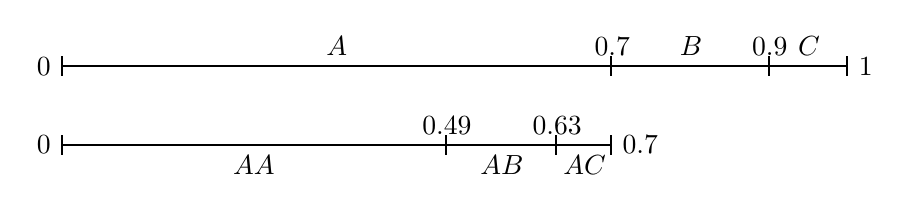
\begin{tikzpicture}
    \draw [|-|,thick] (0,0) node[left] {$0$} -- (7,0) node[midway,
    above] {$A$} node[above] {$0.7$};
    \draw [-|,thick] (7,0) -- (9,0) node[midway, above] {$B$} node[above]
    {$0.9$};
    \draw [-|,thick] (9,0) -- (10,0) node[midway, above] {$C$} node[right]
    {$1$};

    \draw [|-|, thick] (0,-1) node[left] {$0$} -- (4.9,-1) node[midway,
    below] {$AA$} node[above] {$0.49$};
    \draw [-|, thick] (4.9,-1) -- (6.3,-1) node[midway, below] {$AB$}
    node[above] {$0.63$};
    \draw [-|, thick] (6.3,-1) -- (7, -1) node[midway, below] {$AC$}
    node[right] {$0.7$};
  \end{tikzpicture}
  \caption{Wizualizacja kodowania arytmetycznego}
\end{figure}

\subsubsection{Kodowanie całkowitoliczbowe}

Liczbę z kodowania zmiennoprzecinkowego, można zakodować jako zbiór $2^m$
wartości binarnych.
$$
kod(0) = \stackrel{m}{\overbrace{00 \dots 0}}
$$
$$
kod(1) = \stackrel{m}{\overbrace{11 \dots 1}}
$$
$$
kod(0.5) = 1\stackrel{m-1}{\overbrace{00 \dots 0}}
$$

\subsection{Kodowanie Słownikowe}

\subsubsection{Statyczne kodowanie słownikowe}

Zawczasu określamy jakiś słownik słów. Następnie przypisujemy każdemu słowu
kod binarny. W ten sposób kodujemy cały tekst. Takie kodowanie ma sporo wad,
głównie związanych z koniecznością przesyłania słownika oraz z słabą
odpornością na błędy i zmienność danych wejściowych.

\subsubsection{LZ77}

Słownikiem jest zakodowana/odkodowana część tekstu. W ten sposób jesteśmy bardzo
elastyczni w zakresie zmiany danych wejściowych, oraz nie musimy przesyłać
słownika. Kodem jest trójka $(o, l, k)$ gdzie $o$ to przesunięcie, $l$ to
długość, a $k$ to kolejny znak. W ten sposób $(0, 0, n),(1, 1, k)$ dekoduje się
jako "nnk". Proces kodowania jest parametryzowany $n$ i $m$, gdzie $o < n$ i
$l < m$.

\subsubsection{LZ78}

Istnieje osobny słownik, do którego trafiają kolejne słowa. Podczas kodowania
kolejno szukamy w słowniku najdłuższego słowa, które jest prefiksem ciągu
wejściowego. Jeśli nic nie znajdziemy to dodajemy pierwszą literę do słownika,
lecz jeśli znajdziemy taki prefiks, to kodujemy go jako indeks w słowniku,
wraz z kodem następnej litery. Zatem kod $(0,k),(1,a)(2,b)$ oznacza "kkakab",
a słownik $s$ zawiera $s(1)=k,s(2)=ka,s(3)=kab$.

\subsubsection{LZW}

Ta wersja algorytmu pozbywa się drugiego elementu pary z kodowania LZ78.
Z kolei potrzebny jest słownik początkowy zawierający wszystkie możliwe
symbole. Poza tą mała różnicą, algorytm jest identyczny z LZ78.
Zatem ze słownikiem $s$ gdzie $s(1)=a,s(2)=b,s(3)=c$, kod:
$34$ znaczy "cbcb", ponieważ $s(4)=cb$ po pierwszym kroku.

\subsection{bzip2}

\subsubsection{Kodowanie tabelą}

Mając blok danych o długości $n$, tworzymy wszystkie $n$ rotacji tego bloku.
Następnie sortujemy je leksykograficznie. W ten sposób otrzymujemy blok
transformowany.
\newcolumntype{g}{>{\columncolor{gray!50}}c}
\begin{table*}[h]
  \centering
  \begin{tabular}{|g|c|c|c|c|c|}
    \hline
    0 & e & l & l & o & h \\
    \hline
    1 & h & e & l & l & o \\
    \hline
    2 & l & l & o & h & e \\
    \hline
    3 & l & o & h & e & l \\
    \hline
    4 & o & h & e & l & l \\
    \hline
  \end{tabular}
  \caption{Przykład bloku transformowanego dla słowa "hello"}
\end{table*}

\subsubsection{Kodowanie szybkie}

Alternatywnie zamiast tworzenia ogromnej tabeli, wystarczy stworzyć pierwszą
i ostatnią kolumnę. Pierwszą kolumnę tworzy się przez posortowanie słowa
leksykograficznie (w przypadku konfliktu patrzymy na kolejne litery). Ostatnią
kolumnę tworzymy poprzez zapisanie litery poprzedzającej daną literę w
oryginalnym słowie.
\begin{table*}[h]
  \centering
  \begin{tabular}{|c|c|}
    \hline
    e & h \\
    \hline
    \rowcolor{gray!50}
    h & o \\
    \hline
    ll & e \\
    \hline
    lo & l \\
    \hline
    o & l \\
    \hline
  \end{tabular}
  \caption{Wygenerowana pierwsza i ostatnia kolumna dla słowa "hello"}
\end{table*}
Na podstawie tej tabeli zapisujemy numer wiersza, w którym znajduje się
oryginalne słowo, oraz ostatnią kolumnę. W ten sposób uzyskujemy kod
$1$, "hoell".

\subsubsection{Dekodowanie}

Mając tylko te dane, jesteśmy bardzo łatwo w stanie odtworzyć
oryginalne słowo. Najpierw sortujemy nasz kod leksykograficznie, zapamiętując
indeksy.
\begin{table*}[h]
  \centering
  \begin{tabular}{|c|c|c|c|c|}
    \hline
    \rowcolor{gray!50}
    0 & 1 & 2 & 3 & 4 \\
    \hline
    e & h & l & l & o \\
    \hline
    2 & 0 & 3 & 4 & 1 \\
    \hline
  \end{tabular}
  \caption{Tabela dekodowania dla kodu $1$, "hoell"}
\end{table*}
Mając taką tabelę, następnie konstruujemy ciąg, traktując tabelę jak
permutację, zaczynając od indeksu zawartego w kodzie.
W naszym przypadku powstaje permutacja cykliczna $(1, 0, 2, 3, 4)$.
Wykorzystując tę permutację, odtwarzamy oryginalne słowo.

\subsubsection{Move to Front}

Zaczynamy od tabeli liter posortowanych z słowa wejściowego. Następnie
dla każdej litery w słowie, kodujemy ją jako jej indeks w tabeli, a
następnie literę w tabeli przesuwamy na początek. W ten sposób
kodujemy słowo "hello" jako "11203". Taki kod ma mniejszą entropię i
jest łatwiej kompresowalny.

\subsection{V.42bis}

To jest standard, głównie wykorzystywany w modemach, do kompresji i korekcji
błędów w sieciach telefonicznych. Może działać w dwóch trybach: przezroczystym
(bez kompresji) i z kompresją (LZW).

Zaczynamy z słownikiem, o wcześniej ustalonej, negocjowalnej, wielkości.
Wyróżniamy w komunikacji trzy specjalne kody:
\begin{enumerate}
  \item \texttt{ETM} - przejście do trybu przezroczystego
  \item \texttt{FLUSH} - oczyszczenie danych
  \item \texttt{STEPUP} - zwiększenie rozmiaru słownika $\times 2$
\end{enumerate}
Gdy liczba elementów w słowniku przekroczy wartość dozwoloną, wysyłany jest
kod \texttt{STEPUP}. Gdy słownik jest pełny, wysyłany jest kod \texttt{FLUSH}.
W ten sposób, mamy zmienny, dynamiczny słownik, który dostosowuje się do
danych wejściowych po stronie nadawcy i odbiorcy.

\subsection{Kodowanie predykcyjne}

W tekstach naturalnych symbole bardzo często zależą od siebie. Można wykorzystać
informację o prawdopodobieństwach wystąpienia symboli, pod warunkiem wystąpienia
poprzednich symboli. Dla dłuższego okna kontekstowego, kodowanie predykcyjne
jest bardziej skuteczne, lecz wymaga większej ilości pamięci.

\subsubsection{PPM}

Dla kontekstu długości $n$, algorytm PPM polega na stworzeniu drzewa
kontekstowego, które przechowuje informacje o prawdopodobieństwach wystąpienia
poszczególnych symboli. Sczególnym symbolem w tym drzewie jest \texttt{ESC},
który oznacza brak wystąpienia symbolu w danym kontekście. W ten sposób
możemy zbudować drzewo, które pozwala na przewidywanie kolejnych symboli,
które potem można wykorzystać do zbudowania dynamicznego kodowania Huffmana.

\begin{table*}[h]
  \centering
  \begin{tabular}{c|c|c}
    Kontekst & Symbol & Licznik \\
    \hline
    th & \texttt{ESC} & 1 \\
    & i & 1 \\
    \hline
    hi & \texttt{ESC} & 1 \\
    & s & 1 \\
    \hline
    is & \texttt{ESC} & 1 \\
    & - & 1 \\
    \hline
    s- & \texttt{ESC} & 1 \\
    & i & 1 \\
    \hline
    -i & \texttt{ESC} & 1 \\
    & s & 1 \\
  \end{tabular}
  \caption{Przykład drzewa kontekstowego dla słowa "this-is"}
\end{table*}

\subsubsection{CALIC}

Algorytm CALIC jest algorytmem kompresji obrazów, który wykorzystuje
kodowanie predykcyjne. Dla każdego piksela obrazu, wykorzystuje się kontekst
pikseli wokół niego, aby przewidzieć wartość piksela. Chcemy wiedzieć czy w
sąsiedztwie piksela są krawędzie pionowe lub poziome.
\begin{figure*}[h]
  \centering
  \begin{tabular}{|c|c|c|c|}
    \hline
    & & NN & NNE \\
    \hline
    & NW & N & NE \\
    \hline
    WW & W & \color{red} X & E \\
    \hline
  \end{tabular}
  \caption{Kontekst dla algorytmu CALIC}
\end{figure*}
$$
d_h = |W - WW| + |N - NW| + |NE - N|
$$
$$
d_v = |W - NW| + |N - NN| + |NE - NNE|
$$
Następnie na podstawie tych dwóch wartości, tworzymy $\widehat{X}$ i kodujemy
różnicę między $X$ a $\widehat{X}$.

\subsubsection{JPEG-LS}

JPEG-LS to standard kompresji obrazów, podobny do CALIC, który też wykorzystuje
kodowanie predykcyjne.
\begin{figure*}[h]
  \centering
  \begin{tabular}{|c|c|}
    \hline
    NW & N \\
    \hline
    W & \color{red} X \\
    \hline
  \end{tabular}
  \caption{Kontekst dla algorytmu JPEG-LS}
\end{figure*}
\begin{enumerate}
  \item $\widehat{X} = W$
  \item $\widehat{X} = N$
  \item $\widehat{X} = NW$
  \item $\widehat{X} = N + W - NW$
  \item $\widehat{X} = N + \frac{W - NW}{2}$
  \item $\widehat{X} = W + \frac{N - NW}{2}$
  \item $\widehat{X} = \frac{N + W}{2}$
\end{enumerate}
Wśród tych siedmiu możliwości, wybieramy tę, która daje najmniejszą różnicę
między $X$ a $\widehat{X}$ i podobnie jak dla CALIC kodujemy ciąg różnic.

\subsubsection{Poziomy rozdzielczości}

Kodujemy obraz wysyłając średni kolor kwadratów o rozmiarze $2^k \times 2^k$
a następnie różnice między tą średnią a średnią kwadratow $2^{k-1}
\times 2^{k-1}$. Kończymy na pojedynczych pikselach. Różnice między tymi
kwadratami łatwo się kompresuje bo są małe.

\section{Macierzowa notacja kodów}

Macierz generująca, to macierz przez którą mnożymy wektor danych, aby uzyskać
kod. Macierz parzystości to macierz, przez którą mnożymy kod, aby uzyskać
wektor zer. Macierz generująca i parzystości są ze sobą powiązane.
Syndrom to niezerowy wynik mnożenia wektora kodu przez macierz parzystości.

\section{Korekcja błędów}

\subsection{Kody parzystości}

Do każdego bloku danych dodawany jest bit parzystości, który przyjmuje wartość
1, gdy liczba jedynek w bloku jest nieparzysta. W przeciwnym razie
przyjmuje wartość 0. W ten sposób jesteśmy w stanie wykryć jeden błąd w bloku
danych.

\subsection{Algorytm Luhna}

Jest to algorytm wykorzystywany do weryfikacji poprawności numerów z cyfrą
kontrolną. Polega on na pomnożeniu co drugiej cyfry przez 2, wyeliminowaniu
wszystkich liczb dwucyfrowych przez dodanie ich cyfr, a następnie
dodaniu wszystkich cyfr. Na koniec dobierana jest cyfra kontrolna, tak aby
suma wszystkich cyfr była podzielna przez 10.

\subsection{Kod powtórzeniowy}

Kod powtórzeniowy polega na powtórzeniu bloku danych $k$ razy. W ten sposób
jesteśmy w stanie wykryć $k-1$ błędów. Kod powtórzeniowy jest bardzo
nieskuteczny, ponieważ wymaga $k$ razy więcej miejsca na przechowywanie
danych.

\subsection{Współczynnik informacji}

Dla kodu $K$ długości $n$ współczynnikiem informacji nazywamy:
$$
\frac{1}{n}\log|K|
$$
Dla kodu powtórzeniowego $k$ współczynnik informacji wynosi: $\frac{1}{n}$.
Dla kodów parzystości współczynnik informacji wynosi $\frac{n}{n+1}$.

\subsection{Odległość Hamminga}

$$
d(a, b) = \sum_{i = 1}^{n} a_i \ne b_i
$$

Dla kodu $K$ minimalną odległością tego kodu nazywamy minimalną odległość
Hamminga tego kodu. Kod $K$ wykrywa $t$ błędów jeśli jego minimalna odległość
jest mniejsza niż $t$. Z kolei ten sam kod koryguje te błedy jeśli jego
minimalna odległość jest większa niż $2t$.

\subsection{Kody Hamminga}

Kody doskonałe dla korekcji jednego błędu.
Dla długości kodu $2^m - 1$, zapisującego liczby od $1$ do $2^m-1$ dla $m=3$:
$$
G(K) =
\begin{bmatrix}
  1 & 0 & 0 & 0 \\
  0 & 1 & 0 & 0 \\
  0 & 0 & 1 & 0 \\
  0 & 0 & 0 & 1 \\
  0 & 1 & 1 & 1 \\
  1 & 0 & 1 & 1 \\
  1 & 1 & 0 & 1 \\
\end{bmatrix}
$$
Dla wektora informacji $x$, kod liczymy jako: $k(x) = G(K)x$

\subsection{Kody cykliczne}

Kod liniowy nazywamy cyklicznym wtedy i tylko wtedy, jeśli dla każdego słowa
kodowego $v_0v_1 \dots v_n$ cykliczne przesunięcie $v_{n}v_0v_1\dots v_{n + 1}$.
Kod parzystości i powtórzeniowy są kodami cyklicznymi.

Kody cykliczne można reprezentować przy pomocy wielomianów. W takiej
reprezentacji, dodawanie słów kodowych jest równoważne dodawaniu
reprezentujących wielomianów.
$$
a_0a_1\dots a_n \Rightarrow a(x) = a_0 + a_1x + \dots + a_nx^n \in \mathbb{Z}_2
$$

Każdy nietrywialny $(n, k)$-kod cykliczny (kod długości $n$ z $k$ bitami)
zawiera słowo kodowe $g(x)$ stopnia $n - k$. Dla takiego kodu:
$$
G(k) =
\begin{bmatrix}
  g(x) \\
  xg(x) \\
  \vdots \\
  x^{k - 1}g(x) \\
\end{bmatrix}
$$

\subsection{Kody doskonałe}

Binarny $(n, k)$-kod jest doskonały dla $t$ błędów, jeśli ma minimalną odległość
równą $2t + 1$ oraz spełniona jest:
$$
2^{n - k} = \sum_{i = 0}^{t} \binom{n}{i}
$$

Przykładem kodu doskonałego jest kod Golay. Jest to $(23, 12)$-kod.
$$
g(x) = 1 + x^2 + x^4 + x^5 + x^6 + x^10 + x^11
$$
Odległość minimalna tego kodu to $7$ i koryguje $3$ błędy.

\subsection{Burst Error}

Burst error to ciąg błędów, długości $t$. Kod dualny do kodu Hamminga z
$g(x)=1 + x^2 + x^3 + x^4$ jest $(7,3)$-kodem korygującym 2 burst errors.

\end{document}